\documentclass[12pt,a4paper]{article}

\setlength{\parskip}{\baselineskip} % Increase space between paragraphs
\setlength{\parindent}{0pt} % No indentation at paragraph level

\renewcommand{\familydefault}{cmss}
\newcommand{\rp}{\textbf{Raspberry Pi}\xspace}

\usepackage{xspace}
\usepackage[ngerman]{babel} % This is needed for umlauts
\usepackage[utf8]{inputenc} % This is needed for umlauts
\usepackage[T1]{fontenc} % This is needed for correct output of umlauts in pdf
\usepackage[pdftex,breaklinks,colorlinks,
citecolor=blue,
urlcolor=blue]{hyperref}
\usepackage{graphicx}
\usepackage[german]{cleveref} % Prepend \ref with corresponding label
% Use smaller margins
\usepackage[cm]{fullpage}
\usepackage{layout}
\usepackage{float}
\usepackage{wrapfig}
\usepackage{textcomp}
\usepackage{eurosym}

% 'graphicx' configuration
\graphicspath{ {img/} }
\DeclareGraphicsExtensions{.jpg,.png}

% Copy title, author to PDF metadata
\makeatletter
\AtBeginDocument{
  \hypersetup{
    pdftitle = {\@title},
    pdfauthor = {\@author}
  }
}
\makeatother

\begin{document}
% '\layout' to visualize the layout applied
\title{Raspberry Pi}
\author{Hr. Walter, Hr. Ehret und Hr. Ribeaud}
\maketitle

Die \rp Hardware ist ein Einplatinen Computer der von der britischen \href{https://www.raspberrypi.org/}{Raspberry Pi Foundation} gefertigt wird.

Der \rp wurde 2008 ursprünglich entwickelt, Kinder spielerisch in die Welt der Programmierung \& Elektronik einzuführen. Jedoch führte die einfache Handhabung und die fast unendlichen Möglichkeiten zu einer großen Community, die mittlerweile durch alle Schichten und Altersklaßen geht.

Der Name wird wie \textit{raspberry pie} ausgesprochen, das englische Wort für \textit{Himbeerkuchen}. Die \textit{Himbeere} knüpft an die Tradition an, Computer nach Früchten zu benennen, wie etwa \textbf{Apple}. Der \textbf{Pi} stammt aus \textit{Python}, einer Programmiersprache.

Bis Februar 2017 wurden mehr als zwölf Millionen Geräte verkauft. Die Entwicklung des \rp wurde mit mehreren Auszeichnungen bzw. Ehrungen bedacht. Es existiert ein großes Zubehör- und Softwareangebot für zahlreiche Anwendungsbereiche. Verbreitet ist beispielsweise die Verwendung als \href{https://www.youtube.com/watch?v=YPu7oSVbMVo}{Mediacenter}, da der Rechner Videodaten mit voller HD-Auflösung (1080p) dekodieren und über die HDMI-Schnittstelle ausgeben kann. 

\section{Anschlüße und Komponenten}
\label{sec:comp}

Bevor man mit dem \rp richtig loslegen kann, muss man zumindest grob wissen, wo welche Anschlüsse und Komponenten liegen und für was sie gut sind. Deshalb gilt es, alle wichtigen Anschlüsse und Bauteile des \rp richtig zu identifizieren.

\subsection{Aufgabe}

Auf dem unteren Foto des \rp zeichne die folgenden Anschlüsse und Komponenten ein. Antwort befindet sich im \cref{apx:comp} (\cref{fig:rp_ls}).

\begin{figure}[H]
\centering
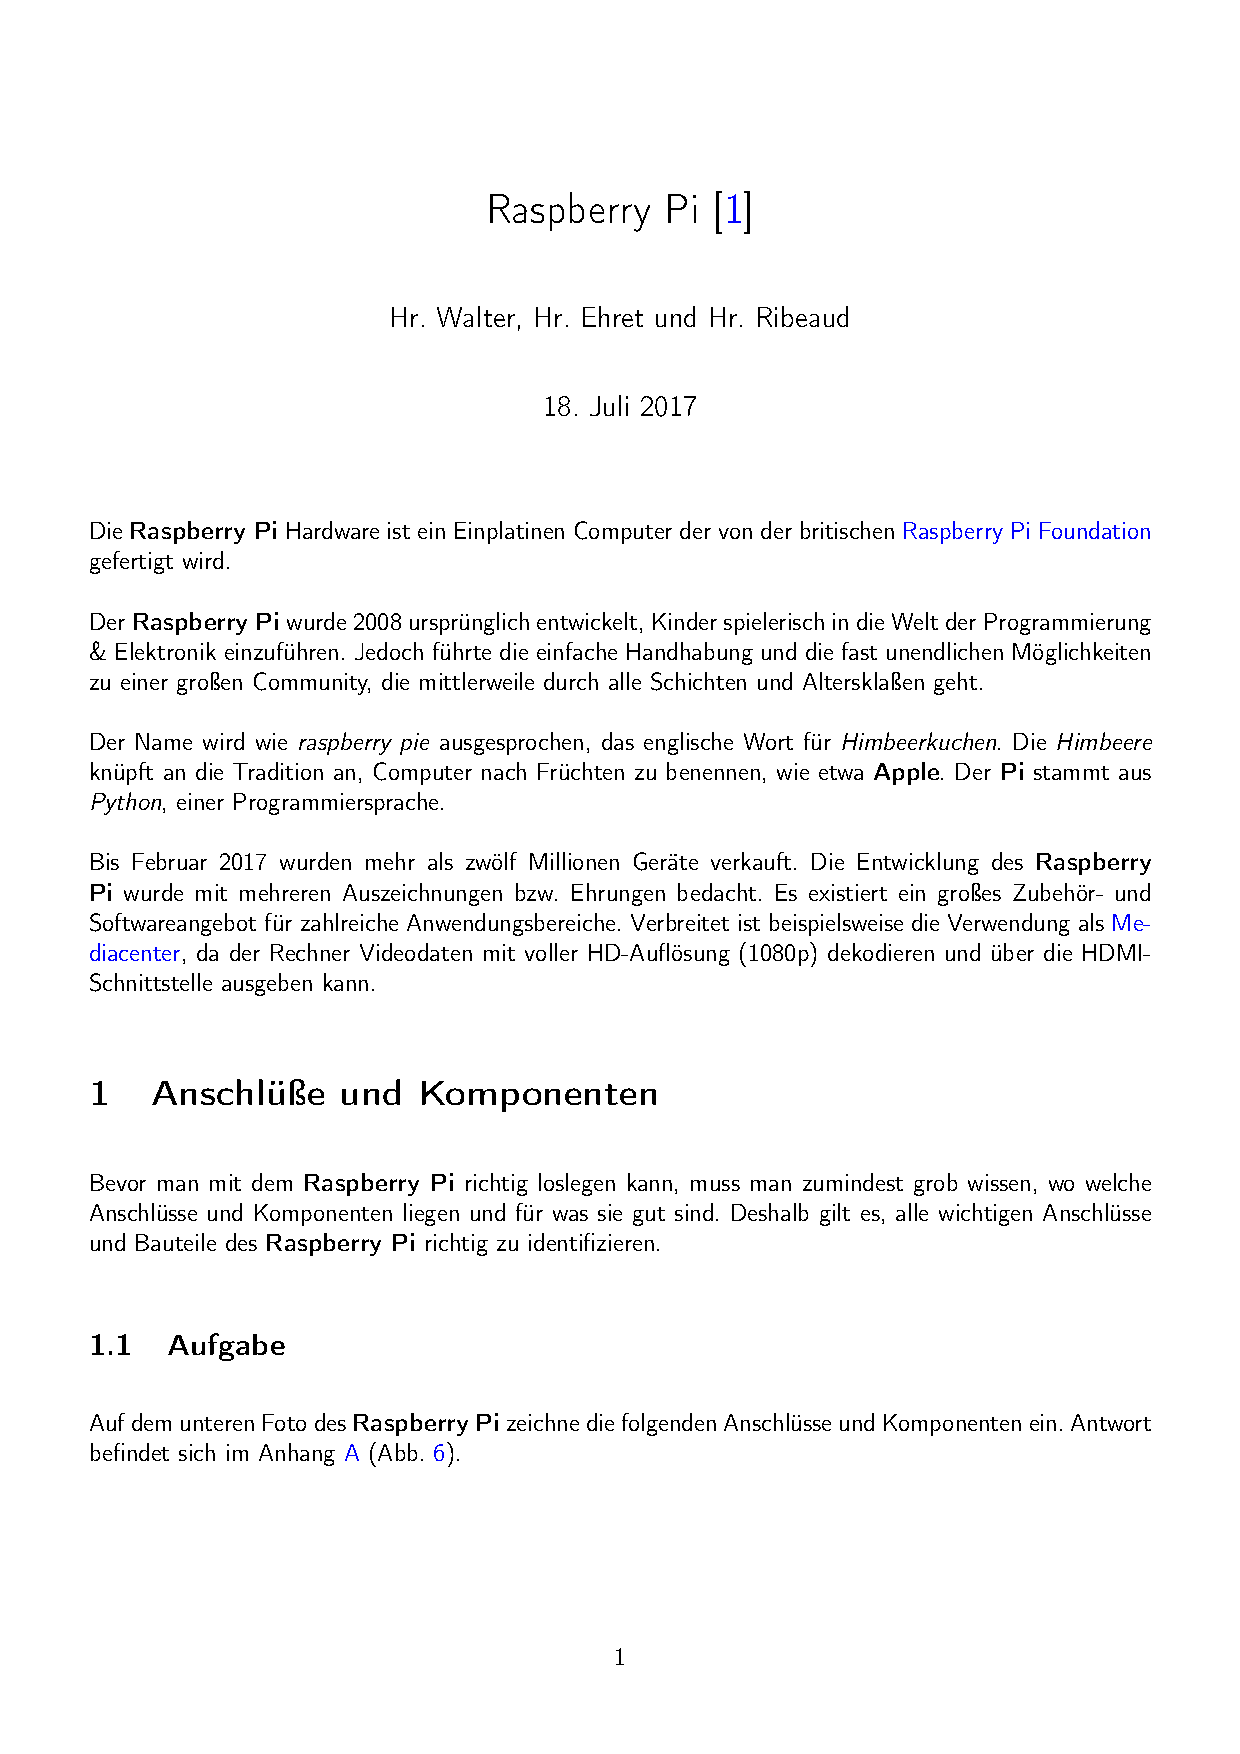
\includegraphics[scale=1.3]{raspberry}
\caption{Raspberry Pi 3}
\label{fig:rp}
\end{figure}

\begin{enumerate}
\item Wo befindet sich der Tastatur- und Maus-Anschluss (USB)?
\item Wo befindet sich der Netzwerk-Anschluss (Ethernet)?
\item Wo befindet sich der Anschluss für einen Bildschirm (HDMI)?
\item Wo befindet sich der Anschluss für Lautsprecher (Klinke)?
\item Wo befindet sich der Anschluss für die Energieversorgung (Micro-USB)?
\item Wo befindet sich der Steckplatz für die SD-Speicherkarte?
\item Wo befindet sich der Steckplatz für Erweiterungen (GPIO)?
\end{enumerate}

\section{Was man noch braucht}
\label{sec:acc}

\subsection{SD Karte}

\begin{wrapfigure}{r}{0.2\textwidth}
  \vspace{-25pt}
  \begin{center}
    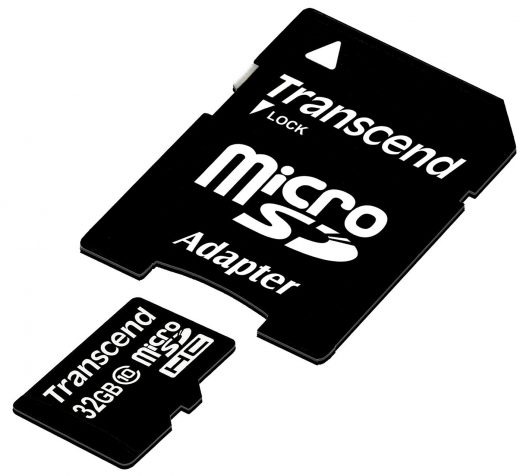
\includegraphics[scale=0.2]{sd_card}
  \end{center}
  \vspace{-25pt}
\end{wrapfigure}

Die \textbf{SD Karte} ist essenziell, denn das \rp kann nicht von einem USB Stick oder Festplatte gestartet werden. Der Geschwindigkeit halber wird eine \textit{Class 10 SD} mit mindestens \textit{8 GB} Kapazität empfohlen. Prinzipiell sind aber bis zu 32 GB möglich. Die minimal benötigte Größe variiert von Betriebssystem zu Betriebssystem zwischen 2 und 6 GB. Falls man eine alte (micro)SD Karte aus der Kamera oder dem Handy hat, kann man diese benutzen.

Vorsicht! Niemals den \textbf{Pi} an dieser Stelle anfassen! Wenn man auf die Mikro-SD-Karte drückt, springt sie heraus. Dann verliert der \textbf{Pi} augenblicklich sein Gedächtnis. 

\subsection{Stromversorgung}

\begin{wrapfigure}{r}{0.2\textwidth}
  \vspace{-12pt}
  \begin{center}
    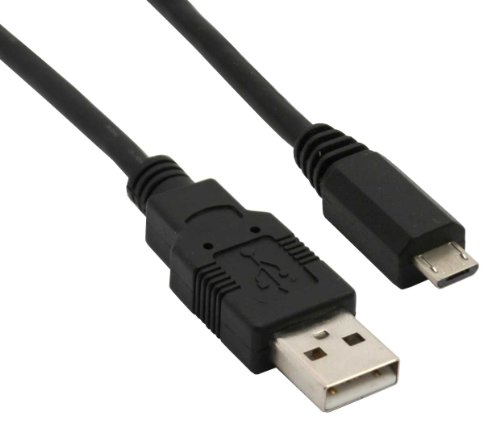
\includegraphics[scale=0.2]{microusb}
  \end{center}
  \vspace{-25pt}
\end{wrapfigure}

Damit der \textbf{Pi} genug Strom bekommt, braucht man ein \textbf{Micro-USB Kabel} mit Netzteil (gibt es auch in einem). Wenn man bereits ein Micro-USB Kabel hat, braucht man nur noch ein USB Netzteil, welches für den Dauerbetrieb geeignet ist und mindestens \textit{1000mA} liefert (auch diese sind separat erhältlich). Der \rp 2/3 sollte mit einem Netzteil, welches \textit{2000mA} liefert an den Strom angeschlossen werden.

\subsection{HDMI Kabel}

\begin{wrapfigure}{r}{0.2\textwidth}
  \vspace{-30pt}
  \begin{center}
    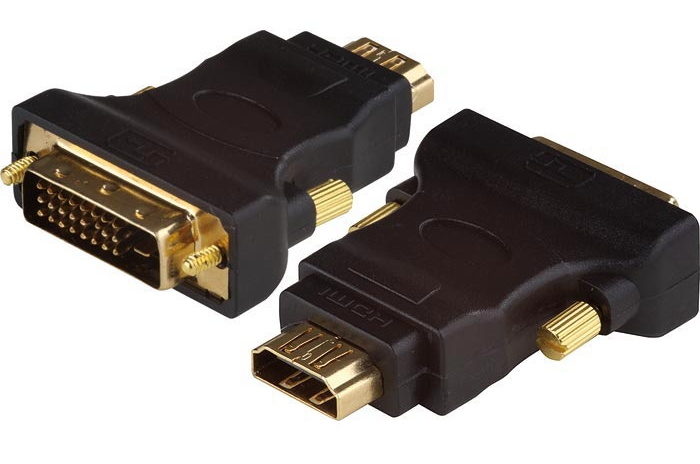
\includegraphics[width=3cm]{hdmi}
  \end{center}
  \vspace{-25pt}
\end{wrapfigure}

Das \textbf{HDMI Kabel} dient dazu, einen Bildschirm anzuschliessen. Wenn der Bildschirm über keinen HDMI Anschluss verfügt (\textbf{DVI} od. \textbf{VGA}), dann muss man sich einen Adapter besorgen.

HDMI steht für \textit{High Definition Multimedia Interface}. Auf Deutsch bedeutet das in etwa Schnittstelle für hochauflösende Multimedia-Geräte. \textit{Hochauflösend} heisst, dass dein Monitor ein sehr gutes Bild mit 1920x1080 Bildpunkten zeigt. \textit{Multimedia} bedeutet, dass Bild und Ton übertragen werden.

\subsection{Maus und Tastatur}

\textbf{Maus} und \textbf{Tastatur} werden via USB angeschlossen. Der \textbf{Pi} bringt 4 USB 2.0 Anschlüsse mit sich.

\subsection{Audio}

Der Ton kann über zwei verschiedene Arten (\textbf{HDMI} und \textbf{3.5mm Klinkenstecker}) ausgegeben werden. Welche man wählt, hängt stark von der Art des Einsatzes ab.

Standardmäßig wird der Ton bei einem über HDMI angestecktem Monitor ausgegeben. Das funktioniert aber nur dann, wenn der Monitor über HDMI auch bekanntgibt, dass er Lautsprecher besitzt. In vielen Fällen funktioniert das aber trotz Lautsprechern nicht. In diesem Fall fehlt der Ton, der wird dann über den analogen 3.5mm Klinkenstecker ausgegeben.

An dem analogen Audio- und Video-Ausgang kann man Kopfhörer oder Aktivboxen anschließen. Aktivboxen sind Lautsprecher mit eingebautem Verstärker und eigener Stromversorgung.

\subsection{Gehäuse}

Da der \textbf{Pi} ohne Zubehör, also auch ohne äußere Verkleidung geliefert wird, kann man ein Gehäuse nachkaufen. Es gibt sie in verschiedenen Formen und Farben (ab 3€ aufwärts). Unbedingt notwendig ist es aber nicht, daher sollte jeder für sich selbst entscheiden, ob er eines benötigt oder nicht.

Was allerdings sehr empfehlswert ist, vor allem wenn der \textbf{Pi} dauerhaft oder längere Zeit laufen soll, sind Kühlkörper. Ein Set besteht aus 3 Kühlkörpern, für die verschiedenen Chips des \textbf{Pi}. Zwar sind die Chips des \textbf{Raspberry} so gemacht, dass sie nicht überhitzen (wie bspw. der Prozessor im Handy), aber dennoch kann die CPU bis zu 45° heiß werden, was nicht besonders zur Langlebigkeit beiträgt. Wer beides will, kann auch einfach auf ein Gehäuse mit Kühlkörpern dabei zurückgreifen.

\section{Hardware}

\subsection{GPIO}

\textbf{GPIO} steht für \textit{General Purpose Input/Output}, heisst auf Deutsch ungefähr \textit{Ein-/Ausgabegerät für viele Verwendungszwecke}. Über diese Schnittstelle können diverse Geräte angesteuert werden (LEDs, Sensoren, Displays, etc).

\begin{figure}[H]
\centering
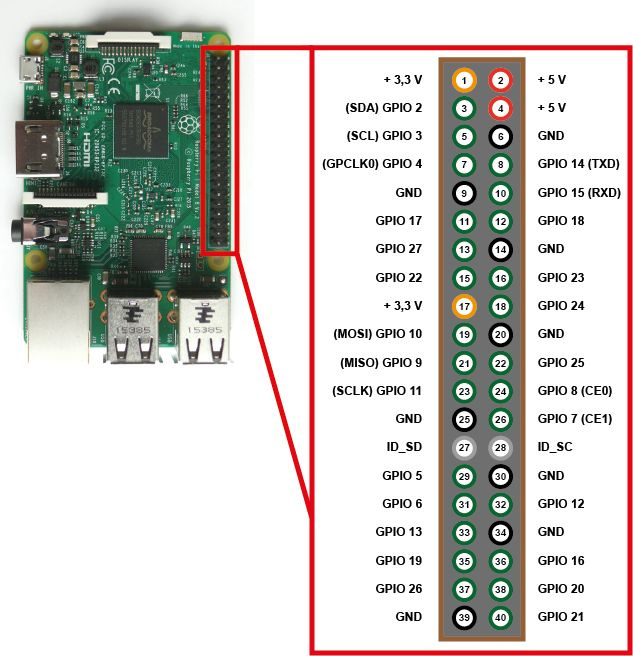
\includegraphics[scale=.5]{gpio}
\caption{General Purpose Input/Output}
\label{fig:gpio}
\end{figure}

\subsection{CSI}

Das \textbf{CSI} erlaubt die direkte Anbindung einer Kamera. Das \textit{Camera Serial Interface} kann eine Kamera mit 5MP ansteuern. Fotos oder Videos sind in diversen Auflösungen möglich.

\begin{figure}[H]
\centering
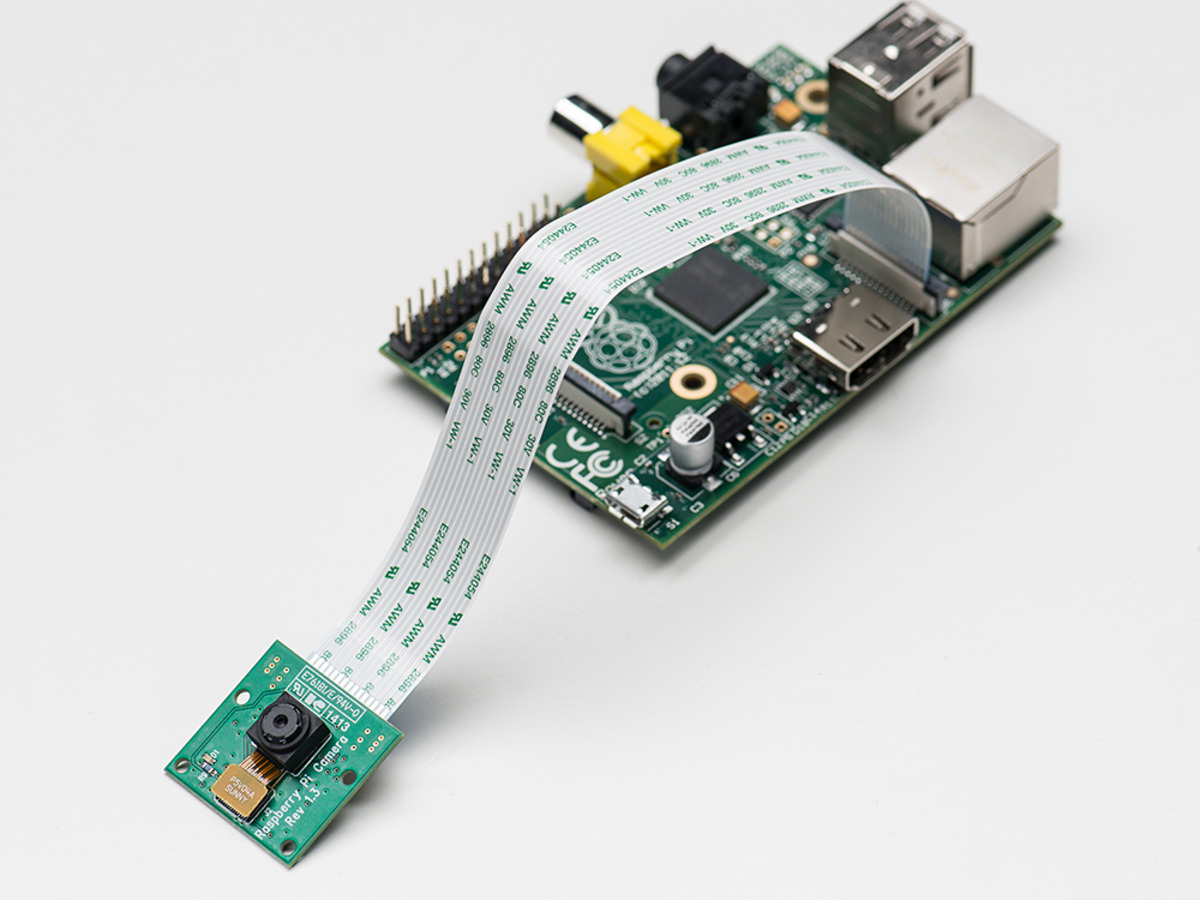
\includegraphics[scale=.8]{csi}
\caption{Camera Serial Interface}
\label{fig:csi}
\end{figure}

\subsection{Antenne}

Das winzige Kästchen ist ein Bluetooth- und WLAN-Modul für Funkverbindungen zum Handy und zum Heimnetz.

\subsection{RJ45-Buchse}

Hier kann man ein LAN-Kabel anschließen, um den \textbf{Pi} mit dem lokalen Netzwerk zu verbinden. Ein LAN (\textit{Local Area Network}) ist ein Netzwerk aus Computern, die über Kabel miteinander verbunden sind. Praktischer ist allerdings ein Funknetz.

\subsection{Aktivitäts-LED}

Die LEDs informiert über den aktuellen Status des \textbf{Pi}. Sie haben folgende Bedeutung:
\begin{itemize}
\item Das grüne, ACT beschriftete Licht blinkt, wenn der \textbf{Pi} auf die SD Karte zugreift.
\item Das rote, PWR markierte Licht leuchtet immer, wenn der \textbf{Pi} über genug Strom verfügt.
\end{itemize}

\subsection{Prozessor (SoC)}

Das ist der Prozessor, das wichtigste Teil eines Computers. Hier werden Daten verarbeitet. Er besteht hauptsächlich aus vielen elektronischen Schaltern, die ständig geöffnet und geschlossen werden und so elektrische Signale über bestimmte Bahnen leiten. In dem \textbf{Pi} ist ein ARM-Prozessor mit einer Taktfrequenz von 1.2GHz. Das bedeutet im Prinzip, dass er in einer Sekunde 1200 Millionen Schaltvorgänge schafft. ARM steht für \textit{Advanced RISC Machines}, auf Deutsch \textit{fortgeschrittene RISC-Maschinen}. RISC wiederum hat nichts mit \textit{Risiko} zu tun, sondern ist eine Abkürzung für \textit{Reduced Instruction Set Computer}, also Computer mit reduziertem Befehlssatz. Das besondere Merkmal von ARM-Prozessoren ist, dass sie wenig Strom verbrauchen. Deswegen findet man sie auch in Mobiltelefonen. Noch etwas: Der Prozessor im Modell 3 hat vier Kerne. Das heisst, es sind eigentlich vier Prozessoren, die zusammen arbeiten.  

\section{Anwendungen}

\subsection{Der \rp als Mediacenter}

Viele ältere oder billige Fernseher besitzen weder einen Internetzugang noch einen USB-Anschluss für Festplatten oder andere Speichergeräte. Ein passend konfigurierter Raspberry Pi rüstet beides preisgünstig nach und bietet zusätzliche Komfort-Funktionen.

Man kann den \rp komplett als Mediacenter einrichten. Ein Mediacenter dieent der Wiedergabe von Medien. Man kann gemütlich auf dem Sofa und sieht sich Fotos und Videos an, hört Musik oder empfängt über das Internet Fernseh- und Radioprogramme.

Das Mediacenter ist nicht für die produktive Arbeit mit dem Computer gedacht. Also: Textverarbeitung, Grafik und Programmieren fallen aus. Man braucht auch keine Tastatur. Eine Maus oder eine Fernbedienung reicht aus.

Um den \rp in ein Mediacenter zu verwandeln, installiert man ein ganz anderes Betriebssystem. Man verwendet OSMC (Open Source Media Center), eine Weiterentwicklung von Kodi. Man kann sich auch ein sogenanntes Media-Set besorgen.

\begin{figure}[H]
\centering
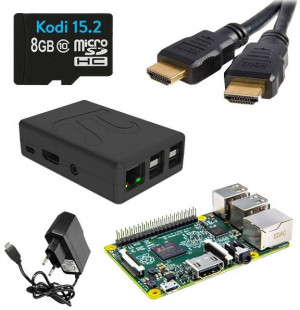
\includegraphics[scale=.8]{kodi}
\caption{\rp als Kodi/XBMC-Mediaplayer}
\label{fig:kodi}
\end{figure}

\subsection{Papp-Lautsprecher mit Google Assistant}

\begin{figure}[H]
\centering
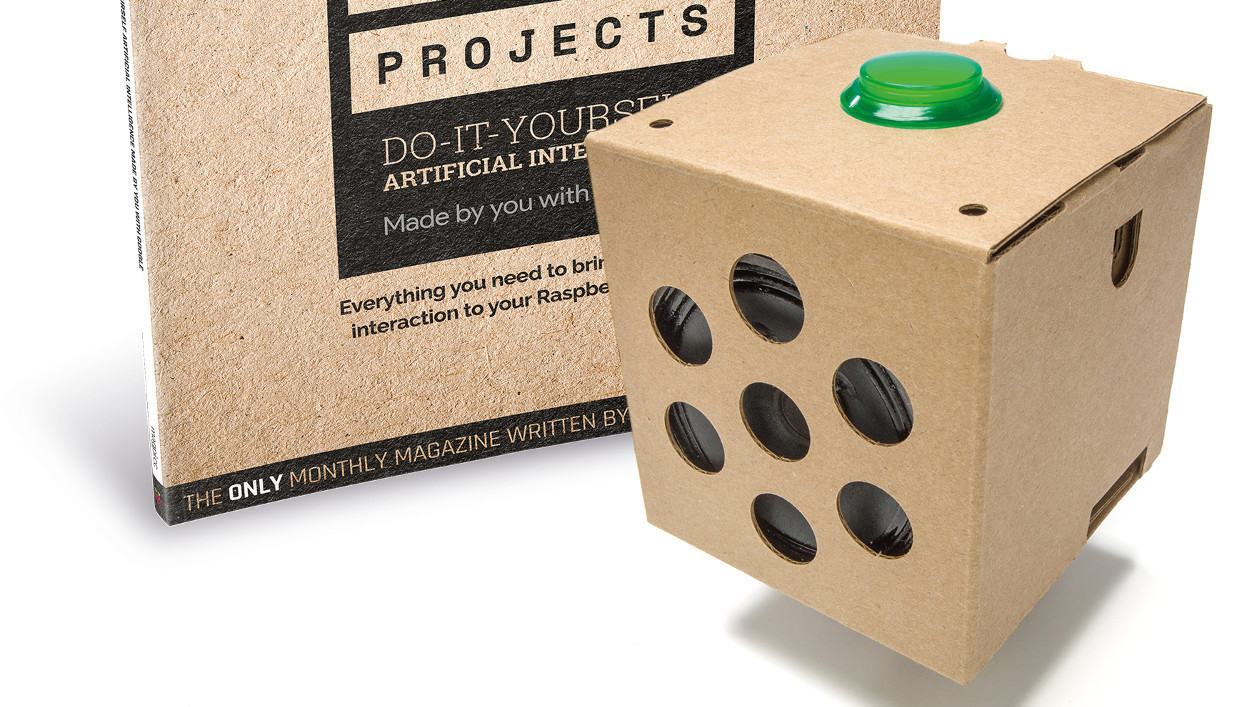
\includegraphics[scale=.3]{aiy}
\caption{Raspberry Pi jetzt mit Google Assistant kompatibel}
\label{fig:aiy}
\end{figure}

\textbf{Google} hat zuletzt eine Schnittstelle bereitgestellt, damit Entwickler auf Funktionen des \textit{Google Assistant (GA)} zugreifen können. Darüber hinaus war der Sprachassistent jedoch bis vor kurzem nur den \textit{Pixel}-Smartphones des Herstellers vorbehalten. Doch das ändert sich nun. Dank der Kooperation mit den Machern des \rp, der gleichnamigen Stiftung, gibt es nun die Möglichkeit, den \textit{GA} auch mit dem \textbf{Pi} zu nutzen.

Tatsächlich gibt es in der englischsprachigen Ausgabe des offiziellen Raspberry-Pi-Magazins, die bereits ausverkauft ist, sogar einen Bausatz, um aus dem \textbf{Pi} einen Google-Home-Ersatz zu machen, samt Lautsprecher, Mikrofon, Papp-Box, Kabeln und einer Schritt-für-Schritt-Anleitung, sowie natürlich der notwendigen Software. Sie sind dann in der Lage, das Gerät ähnlich wie Amazons Alexa als Lautsprecher zu nutzen, der Ihnen über alles Mögliche Auskunft geben kann. Oder aber Sie nutzen die Schnittstelle zur Spracherkennung darüber hinaus noch weiter und programmieren eigene Befehle. Stellen Sie sich vor, dass Sie darüber einen fahrbaren oder zumindest beweglichen Roboter auch per Sprachbefehl steuern.

Was alles in dem Paket enthalten ist, wird im nachfolgenden \href{https://www.youtube.com/watch?v=7WtSdWSv7uo}{Video} (engl.) erklärt.

\subsection{Mit dem \rp die Wohnung überwachen}

Überwachungskameras aus dem Einzelhandel kosten oft viel Geld, bieten wenig Funktionen oder erweisen sich im Einsatz als unflexibel. Mithilfe des \rp umgeht man alle diese Nachteile und erweitern bei Bedarf das System unkompliziert um weitere Features. Man braucht nur noch eine Kamera und die Software \textbf{Motion}.

Eine ausführliche Anleitung findet man zum Beispiel \href{ttps://www.pcwelt.de/1925151/}{hier}.

\clearpage
\appendix
\makeatletter
\def\@seccntformat#1{Anhang~\csname the#1\endcsname:\quad}
\makeatother

\section{Anschlüße und Komponenten}
\label{apx:comp}

\begin{figure}[h]
\centering
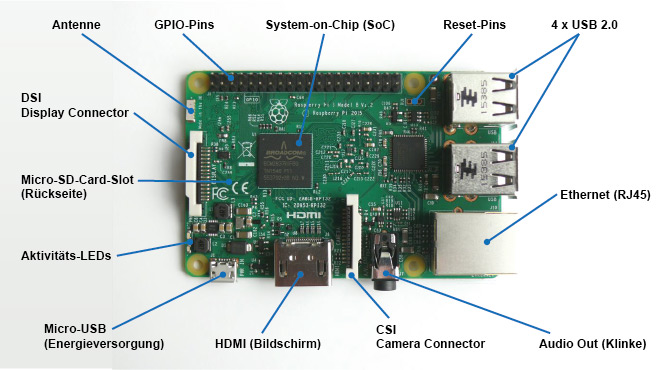
\includegraphics[scale=0.7]{raspberry_loesung}
\caption{Raspberry Pi 3}
\label{fig:rp_ls}
\end{figure}

\end{document}
